\documentclass{article}

\usepackage[utf8]{inputenc}
\usepackage[top=2cm, left=2cm, right=2cm, bottom=2cm]{geometry}
\usepackage{subfig}
\usepackage{graphicx}
\usepackage{tablefootnote}
\usepackage{subfig}

\title{Homework 7 - Feature selection \\
        \vspace{5px} \large UTFPR - CPGEI - Data Mining \\
        Prof. Dr. Heitor Silvério Lopes}
\author{Vinícius Couto Tasso}
\date{November, 2019}

\begin{document}

\maketitle

\section*{Gene-drug test dataset}

This dataset contains data about the chemosensitivity of 733 proteins (instances) to 119 different drugs (attributes). The proteins are divided into 6 functional groups: \textit{Transporter, Double, Channel, ADMAS, RGS, and Contig}.

Since there is a considerable amount of attributes, filters were applied to rank features and select the 5 most relevant attributes, reducing the data dimensionality. The classification was performed for each set of features using J48. Results are shown in Table \ref{tab:gene_drug}.

\begin{table}[htbp]
    \centering
    \begin{tabular}{c|c|c|c|c|c|c}
         Classifier &  \# features & Filter & Tree size & TP Rate & FP Rate & AUC\tablefootnote{Area under the ROC curve} \\ \hline
         J48 & 119 & None & 251 & 0.332 & 0.269 & 0.533  \\
         J48 & 5 & Information Gain Ratio & 183 & 0.352 & 0.318 & 0.504 \\
         J48 & 5 & Gini & 281 & 0.344 & 0.332 & 0.497 \\
         J48 & 5 & Chi-squared & 173 & 0.367 & 0.320 & 0.507 \\
         J48 & 5 & ANOVA & 221 & 0.369 & 0.285 & 0.549 \\
    \end{tabular}
    \caption{Classification results for different sets of features}
    \label{tab:gene_drug}
\end{table}

Although the output of the filters ranking was different for every filter, meaning a different set of features for every experiment, the results were similar and so was the decision tree dimensions. Dimensionality reduction did not improve by much the classification performance or the comprehensibility of the classifier. 

A possible explanation for this is the fact that the problem, with these attributes, is just very difficult. Maybe identifying the functional group the protein is part of has nothing to do with its chemosensitivity to the drugs tested and, even if it has, this means that this sensitivity alone is not enough to determine the functional group.

\section*{Phoneme dataset}

This dataset was built to aid the development of a voice recognition system of French and Spanish. The dataset contains 5 features, corresponding to the amplitude of the first five harmonics of the sound of each subject pronouncing different phonemes. The dataset contains 2 classes: 0, the majority class with 3818 instances, and 1, the minority class with the remaining 1586, totaling 5404 different samples collected for the dataset.

To establish a baseline, classification was made with J48 with a confidence factor of 0.1 and 200 minimum objects per leaf. Due to the fact that there are very few attributes, the result tree is reasonably small, with just 7 leaves and 13 nodes. Results are shown in Table \ref{tab:phoneme_baseline} and the confusion matrix is presented in Figure \ref{fig:cfmatrix_ph1}.

\begin{table}[htbp]
    \centering
    \begin{tabular}{c|c|c|c|c|c}
         Class &  TPR & FPR & AUC & CCI\tablefootnote{Correctly Classified Instances} & ICI\tablefootnote{Incorrectly Classified Instances} \\ \hline
         0 & 0.880 & 0.450 & 0.764 & 3358 & 460 \\
         1 & 0.550 & 0.120 & 0.764 & 873 & 713 \\
    \end{tabular}
    \caption{Classification results for the baseline experiment}
    \label{tab:phoneme_baseline}
\end{table}

\begin{figure}
\centering
\subfloat[J48 classification]{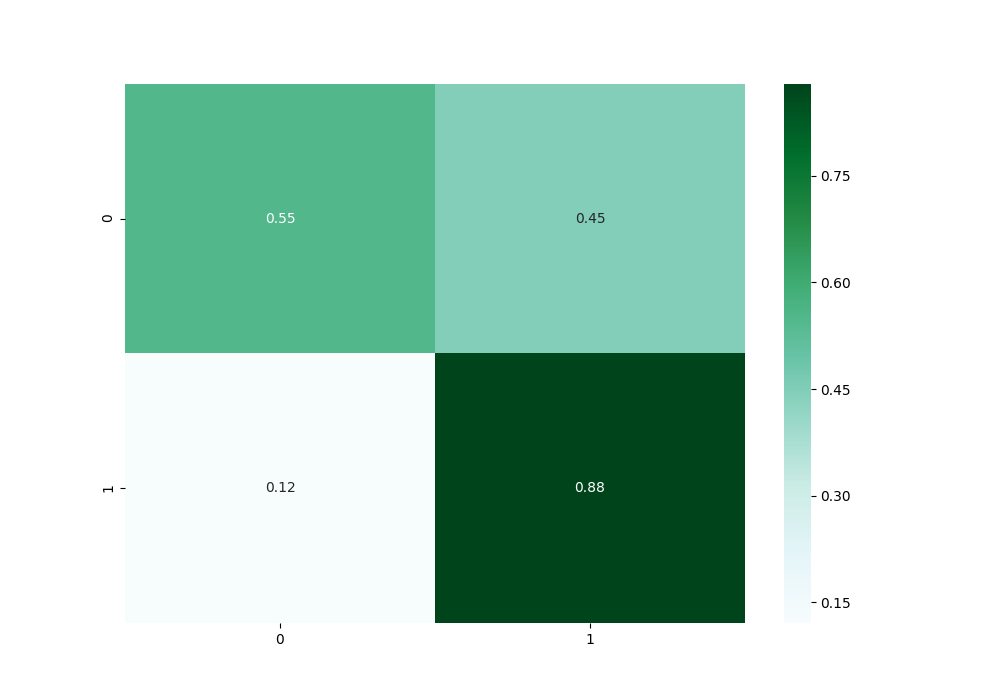
\includegraphics[width=0.5\textwidth]{cfmatrix_ph1.png}} 
\subfloat[K-means clustering]{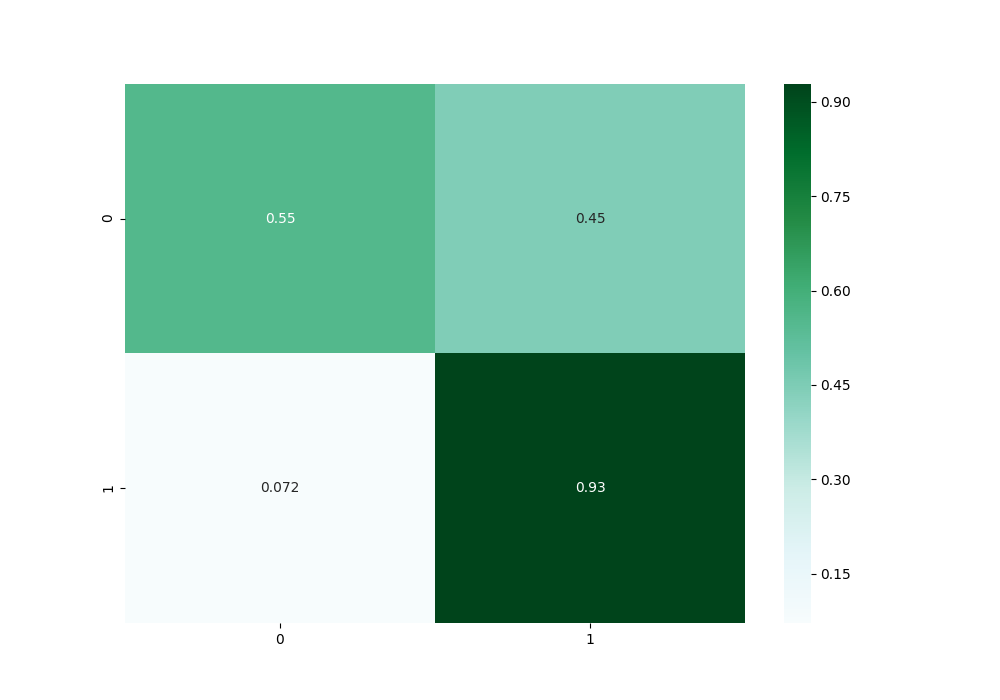
\includegraphics[width=0.5\textwidth]{cfmatrix_ph2.png}}
\caption{Confusion matrix} 
\label{fig:cfmatrix_ph1}
\end{figure} 

Since the dataset is unbalanced, with the majority class representing more than two-thirds of the whole dataset, it is expected that classification results would reflect the disbalance. Further inspection of the attributes shows that only 2 of them are enough to provide reasonable data separability, as shown in Figure \ref{fig:ah1_vs_ah5}.

\begin{figure}[htbp]
    \centering
    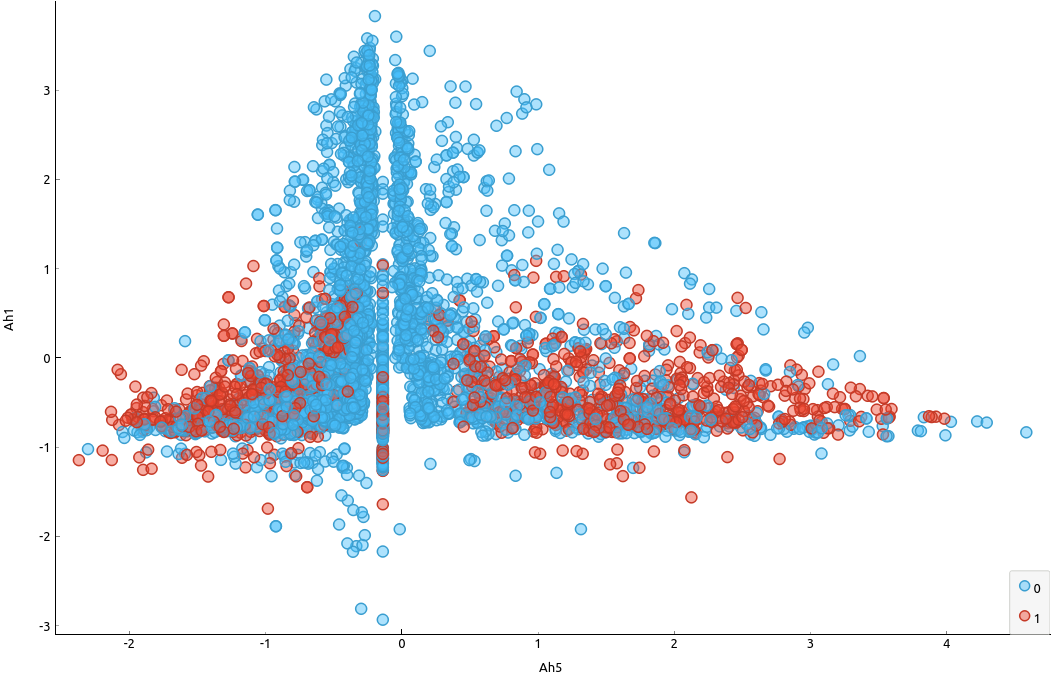
\includegraphics[scale=0.4]{ah1vsah5.png}
    \caption{Scatter plot of the first harmonic (ordinate) versus the fifth harmonic (abscissa)}
    \label{fig:ah1_vs_ah5}
\end{figure}

K-means clustering was also employed to compare the J48 classification results. The evaluation used clusters as classes and showed that the method had 1814 (33.56\%) incorrectly clustered instances. Figure \ref{fig:cfmatrix_ph1} presents the confusion matrix of said evaluation.

Principal Component Analysis (PCA) was applied to reduce data dimensionality with a covered variance of 90\%. The result was 4 features (PC1, PC2, PC3, and PC4), resulted from linear transformations of the original ones. Given that the features are different, Figure \ref{fig:pc1_vs_pc2} presents a scatter plot of the two Principal Components that better represents the variance seen on the data.

Compared to Figure \ref{fig:ah1_vs_ah5}, it is easy to see that, with these transformed features, the data is much better separated. Class 1 instances are closer together and a single vertical line, orthogonal to the X-axis, that crosses the origin is able to give a pretty decent separation, with most of Class 1 contained in the left side, and the majority of the Class 0 at the right side.


\begin{figure}[htbp]
    \centering
    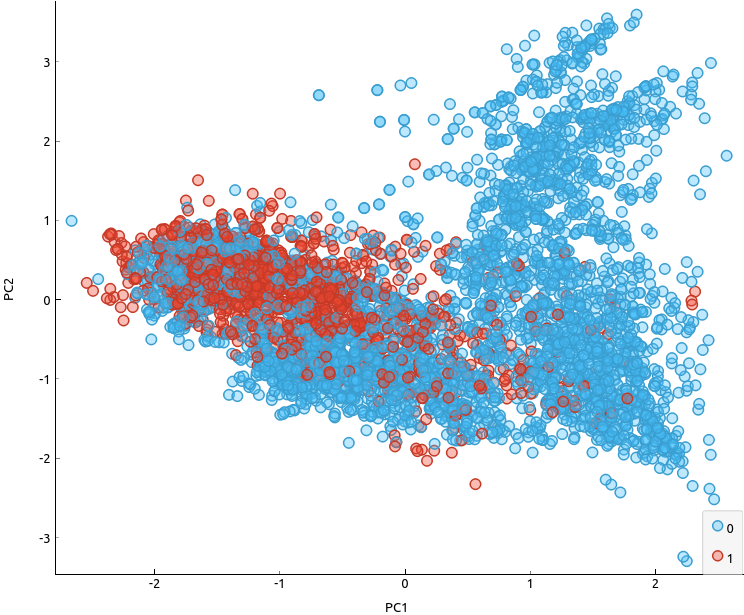
\includegraphics[scale=0.5]{pc1vspc2.png}
    \caption{Scatter plot of the first Principal Component versus the second}
    \label{fig:pc1_vs_pc2}
\end{figure}

Both the classification with J48 and K-means were performed on the data with the transformed attributes. J48 generated a smaller tree, easier to analyze, containing only 9 nodes and 5 leaves. Although the tree complexity is smaller than the previous one, it is important to note that these attributes do not represent the same features of data that the original attributes did. Since the Principal Components are a result of the transformation of the original attributes (five first harmonics), their semantic meaning has been lost in the process. 

Table \ref{tab:phoneme_pca} presents the classification results of the new approach. In comparison with classification using the original features, Class 1 results had a significant improvement, while Class 0 had a negligibly worse result. Figure \ref{fig:cfmatrix_ph_pca} shows the confusion matrix of the classification, that illustrates very well the improvements with the darker colors more present along its principal diagonal. 

\begin{table}[htbp]
    \centering
    \begin{tabular}{c|c|c|c|c|c}
         Class &  TPR & FPR & AUC & CCI & ICI \\ \hline
         0 & 0.875 & 0.354 & 0.796 & 3341 & 477 \\
         1 & 0.646 & 0.125 & 0.796 & 1024 & 562 \\
    \end{tabular}
    \caption{Classification results for the PCA experiment}
    \label{tab:phoneme_pca}
\end{table}

aHowever, the clustering results were very similar and did not seem to benefit very much from the transformation of features, as seen in Figure \ref{fig:cfmatrix_ph_pca}. The evaluation was once again done with clusters as classes.

Overall, PCA was beneficial for the classification task, increasing the classification accuracy in roughly 3 percentage points. The transformed set of features did not include the last feature of the dataset (fifth harmonic) and successfully diminished the data dimensionality. Notwithstanding, when it comes to knowledge discovery, the transformation of features makes it very hard to encounter novel relations of cause and consequence between the data class and its features, since the new features do not represent the same physical characteristics of data.

\begin{figure}
\centering
\subfloat[J48 classification]{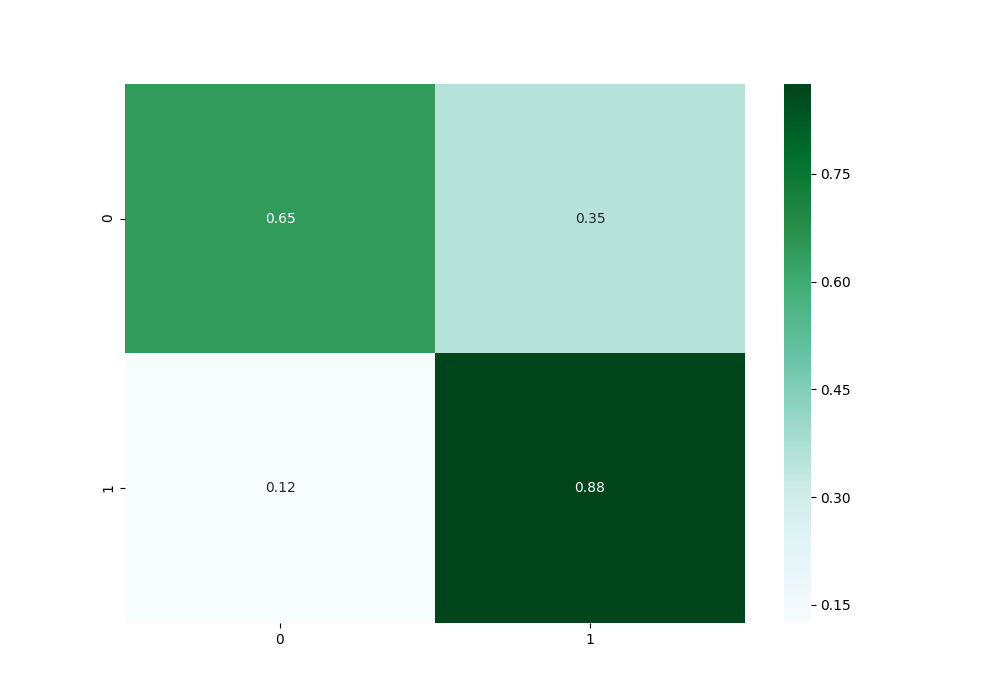
\includegraphics[width=0.5\textwidth]{cfmatrix_ph_pca.png}} 
\subfloat[K-means clustering]{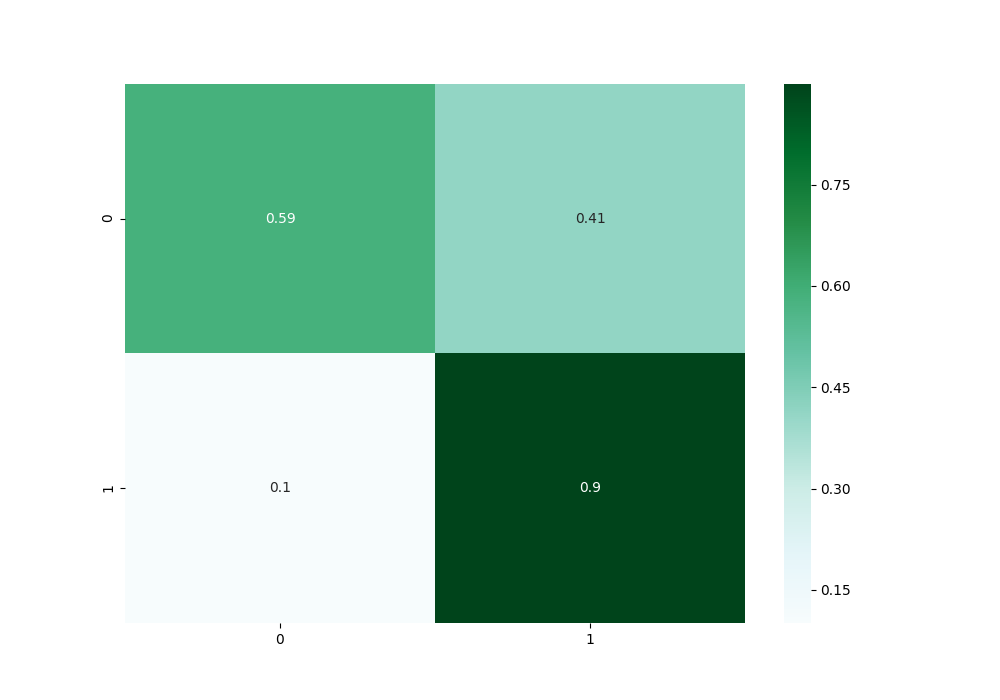
\includegraphics[width=0.5\textwidth]{cfmatrix_ph_pca2.png}}
\caption{Confusion matrix} 
\label{fig:cfmatrix_ph_pca}
\end{figure} 


\end{document}

